\documentclass[a4paper,10pt]{article}
\usepackage[utf8]{inputenc}
\usepackage[english]{babel}
\usepackage{indentfirst}
\usepackage{listings}
\usepackage{graphicx}
\usepackage{blindtext}
\usepackage{enumitem}
\usepackage{hyperref}
\usepackage[top=2.0cm,bottom=2.0cm,left=2.0cm,right=2.0cm]{geometry}
\pagestyle{headings}
\title{Mobile Embedded Group Project}
\author{Ilias Boulif, Jérémy Bricq, George Rusu}
\date{\today}
\begin{document}
\maketitle
\section{Introduction}

The aim of this project is to propose an implementation of an IoT network using \textit{Rime} where the sensor data is published through an MQTT-Rime gateway to normal MQTT subscribers. To achieve that we have implemented as requested by the project's statement, a tree-based routing protocol using Rime and an MQTT-Rime gateway.

Firstly, we are going to explain the general structure of our system. Secondly, we are going to present and explain the different messages exchanged in a normal run. Then, we will explain the organization and the routing in our environment. We will speak briefly about our gateway and MQTT subscriber implementation. And finally, we will discuss about the optimizations we managed to implement.

The implementation source code of this project is available in our Github repository which can be accessed using this \href{https://github.com/georgesrusu/MobileEmbeddedComputing}{link}.


\section{General structure of our system}
Our infrastructure is divided in 2 sides: over air network (root and sensors) and wired network. This infrastucture is illustrated in Figure \ref{fig:fig1}.

\begin{figure}[!htb]
\centering
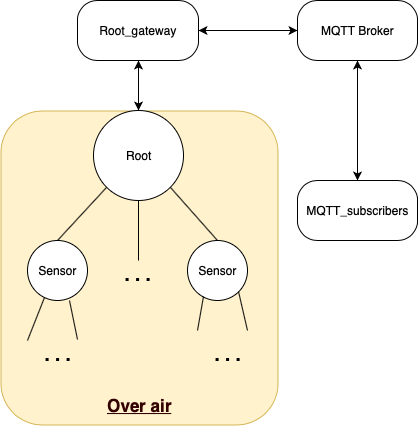
\includegraphics[scale=0.5]{./img/structure.png}
\caption{Representation of our structure}
\label{fig:fig1}
\end{figure}


The over air side (yellow part) is composed of one root node and a number of sensor nodes. When the sensor nodes have some collected data to publish, they will forward the information all the way up to the root. In order to accomplish that, there exists only one path from each sensor to the root. This is achieved by the fact that, each sensor chooses a parent according to its rank. In our system, the rank corresponds to the number of hops from the node to the root. Hence, when choosing a parent, each sensor will look for the parent with the lowest rank, in other words, with the shortest path to the root. \\

Once arrived at the top of the tree, the information is forwarded to the rime gateway which will publish all the sensor's information to the MQTT broker. The most important component is the root of the tree because he is responsible for the transmission of the data from the air network to the wired network. Once the data has been published in the broker, any MQTT subscriber can subscribe to topics in order to receive data of interest. \\

In our system, the nodes communicate together by sending different kind of messages that will be explained later in this document (see Section \ref{msgFormat}). Some of these messages are used to ensure a good working of the system. Indeed, the network is built as such to keep sending information up to the root even if a node is moved or deleted, this will be explained in the Section \ref{routing}. \\


Regarding the collection of data from the sensors by the root, there are two modes which describe the system's behaviour. The root receives some configuration messages, respectively the mode and the number of subscribers through the gateway.  He forwards the received configuration to the sensor nodes by the mean of the discovery and alive response packets, this will be explained in the Section \ref{gateway}. \\

Lastly, we will explain in Section \ref{subscriber} our MQTT subscriber implementation which is basically a simple tool to subscribe to several or all topics in the broker.



\section{Message format}
\label{msgFormat}
In our implementation we have 3 packets structures. The node interprets the packet according to his type. We will explain each kind of packets and discuss the different types used by nodes to communicate between them.

\paragraph{Description of \textit{packet}}
\begin{enumerate}
\item Type : [DISCOVERY\_REQUEST, DISCOVERY\_RESPONSE, ALIVE\_REQUEST, ALIVE\_RESPONSE]
\item Rank : The rank of the transmitting node
\item Mode : The sent mode [DATA\_ON\_CHANGE, DATA\_PERIODICALLY] - by default, data periodically 
\item HaveSubscriber : Boolean that indicates if someone is subscribed to some topics
\end{enumerate}

\paragraph{Description of \textit{data\_packet} }
\begin{enumerate}
\item Type : [SENSOR\_DATA]
\item NodeSrc :  The source node transmitting the data
\item NodeRank : The rank of the node source
\item DataTemp : The temperature data
\item DataADXL : The accelerometer data
\end{enumerate}

\paragraph{Description of \textit{data\_packet\_aggregate} }
\begin{enumerate}
\item Type : [SENSOR\_DATA\_AGGREGATE]
\item numberPacket : The number of contained packets
\item packet1 :  The first packet
\item packet2 : The second packet
\end{enumerate}

\paragraph{DISCOVERY\_REQUEST:}  This message is used when a node starts and his rank is equal to 0. The node will send a broadcast discovery request to find a parent connected to that network. This message is used even when connected to a parent, in order to search the environment for a better parent, if there is one.

\paragraph{DISCOVERY\_RESPONSE:} After receiving a discovery request, this message will be used to respond in unicast. 

\paragraph{ALIVE\_REQUEST:} Once a node has its parent, he will use an alive request to continuously ping his parent in order see if he is still available.

\paragraph{ALIVE\_RESPONSE:} When a node receives an alive request, he has to reply with an alive response to his child to validate his presence. 

\paragraph{SENSOR\_DATA:} This message is used for sending sensors data. 

\paragraph{SENSOR\_DATA\_AGGREGATE:} A sensor data aggregate packet is a packet that contains 2 sensors data packets. This has been implemented as one of our optimizations.

\section{Network organization and routing}
\label{routing}
In order to explain more easily the network organization, let us define the root node as a parent and the sensor as a child. We should note that each sensor will also be a parent at his turn for his children except the root which will only be parent (tree structure).

So let us start from the beginning when the mote network is empty and the root/parent is started and is waiting for messages. Once the first sensor/child is up and running, he will start to search for a network, and thus search for a parent to attach to. He will send using the broadcast channel a discovery request to find a parent. In order to have this working properly, we define that the root node will always have the same rank which is 1 (no other node is allowed to have a rank of 1). When the root/parent receives a discovery request packet, he will reply with a discovery response containing his rank in unicast. The node/child that has made the request receives now the response, checks the received rank (parent+1) and if it is better than his actual rank, he will change or not his parent and hence his rank. This first message exchange is illustrated in Figure \ref{fig:bd}. We should note that even when connected to a parent, the child will still keep sending discovery request in order to search the environment for a better parent, if there is one. The lowest the rank is (except a rank of 0), the nearest the node is to the root (root's rank=1).\\

\begin{figure}[!htb]
\centering
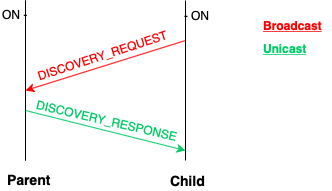
\includegraphics[scale=0.6]{./img/discovery.png}
\caption{First communications between nodes.}
\label{fig:bd}
\end{figure}

Once the child got his parent, the alive exchange is starting. This is illustrated in Figure \ref{fig:alive}. The child will create an alive request packet and send it to his new parent. The child will also start counting the number of alive request packet send without response. So for example after having sent 4 times an alive request packet and not having receive any reply from the parent, the child will reset his parent and start looking again for a new parent. This allow our network to self-rearrange when a node is moved or deleted. However this is time consuming, we need time for our system to converge to a desired state. Back to our alive message exchange, when the parent receives an alive request, he will reply with an alive response to validate his presence. The message is containing the rank, the mode of data transmission desired and the number of MQTT subscribers (we will come back to those later in this document).\\

\begin{figure}
\centering
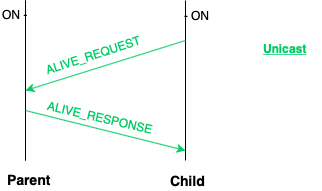
\includegraphics[scale=0.6]{./img/alive.png}
\caption{Keep alive communication between child and parent.}
\label{fig:alive}
\end{figure}

After having received the first alive response from his parent, the child will use the contained information (mode \& subscriber) to start pushing data toward the root of the tree. We should note that when there is no subscriber, the sensors will not start pushing data to the root. Also, if the rank of a sensor node is not greater than 1,  meaning that the node has not yet a parent, then the node will not send any data. For sending the data, the node will create a sensor data packet and send it to his parent. When his parent will receive the sensor data packet, he will try to aggregate the packet in a sensor data aggregate packet in order to decrease the number of transmitted message toward the root. This will also be explained in more details in Section \ref{opti}. Finally, when the data arrives at the root node, it will be forwarded through serial to the gateway which will do the rest in order to publish the data correctly (topics).

\section{Gateway}
\label{gateway}

Once the sensor data arrive at the top of the tree, the root node has to forward it to the gateway in order to be published in the MQTT-broker. In order for this to work, we decided to implement the time gateway using Python3. Regarding the communications between the root node and the gateway, we used the Cooja's plugin \emph{serial2pty} to create a serial communication between them. Basically what it happening, when the root receive a data, he is going to print the data on the serial while the gateway will continuously be reading that serial. When a data is read, the gateway will make a call to the API of the Mosquitto Broker in order to publish the received data according to the related topic, either temperature or acceleration (ADXL). As asked in the assignment, the gateway should act as a management console for the air network (sensors). So we managed to run the gateway in such a way (involving threading) that it accepts input at any time. The input is either 0 or 1 and is for the sending mode of the data. We defined the 0 as the DATA\_ON\_CHANGE and we defined 1 for the mode DATA\_PERIODICALLY. We also defined a default mode which is 1. Thus using our console allows to change the mode from 0 to 1 or vice-versa and unlimited times without having to stop and relaunch the gateway. The mode configuration propagation will be explained in Section \ref{opti} when we will speak about the first optimization (subscribers).


\section{MQTT-Subscriber}
\label{subscriber}
In order to be able to test our MQTT broker and the data being published, we decided to implement a simple MQTT subscriber that is taking as command line argument the topics, if none, then all topics, and will subscribe to the given topics in the MQTT broker.


\section{Optimizations}
\label{opti}
In this project, we implemented the requested optimizations but also we tried to design our network to be as much efficient as possible.  So let us start by explaining the requested optimizations.

The first asked optimizations was that the sensors nodes should not send any data if there is no subscriber. We managed to implement this by using the alive communications, a default value and the trick given in the project assignment. So basically what we are doing is that by default there are no subscriber. Our gateway has subscribed to the MQTT topic \emph{SYS/broker/clients/active}. We should note that here the subscriber number 1 is the gateway so we are only interested when the number of subscriber is $\geq 2$. When a real subscriber (using our MQTT-subscriber.py script) is actif, the gateway receives the number of active clients, if the number is greater or equal to 2 we forward it to the root node which is changing the default subscriber value from 0 to 2. The number of subscribers will be forwarded towards the leafs of the tree using the alive packets. Remember that earlier in this document we spoke about the alive\_response packet and that it contains a variable related to the number of subscribers and the sending modes. Well this is the trick. Using alive response messages (from parents to children) we are not only checking the parent presence but also propagating configuration messages to sensor nodes. And this is how we managed to propagate mode and subscriber configuration. We should not forget to mention that if a node has no parent, there will be no data sent! Once a node get a parent, the rank's node will be greater of 1 than his parent rank, but the node will start the alive messages exchange containing the number of actives subscribers from his parent (response) and finally according to the received information, the node will start or not pushing data information into the network. \\

The second asked optimizations was to aggregate data packets. For that optimization we created the sensor data aggregate packets which is basically a bigger packet than can contain up to 2 data packet. So when a node receives a sensor data, he will create an aggregate packet and wait as long as 2 runicast packets are received. If before that time, the packet aggregate is full, meaning that in the meantime another sensor data packet has been received, the node will immediately send the  aggregated packet toward the root. On the other side, if after that time,  the packet aggregate has not been filled, the packet will be send half-full. And this is leading us to another optimization: we are aggregating half-full data aggregate packet. If an aggregate packet is sent half-empty, the next node on the path to the root, will take the packet, look at the number of packets aggregated into (remember the numberPacket field in the struct) and if it is equal to 1 (only 1 paquet, half-empty) add if available, a sensor data packet. The goal is that no aggregate packet will arrive at the root half-full. 

And finally, the biggest optimization we think is that we managed to have the least message structures, the least message types and of course the least message exchange. This can clearly be observed: we used the same struct of packet for the discovery and alive communication. We could have done this with one struct per message type. Also, we discovered during the testing phase of our prototype that the more messages are exchange the more transmissions errors we got (runicast retransmissions, runicast time-out) and this is why we tried to have the lowest number of messages transiting through the network but some messages cannot just be suppressed.

\section{Conclusion}

As a conclusion, we can say that developing such an IOT network is clearly not an easy task. Firstly it require using a low level machine language which in our case is C and which make use of pointers (easy to get lost into). Secondly, as the root node and the sensor nodes are based on threads sometimes debugging can be difficult: chronological order of events are not always as expected. Thirdly, because of that, the systems need time in order to converge into the desired state. But in the end, it has been a great introduction into the IOT world !

\end{document}